\section{Exploring One-Variable Data}

Much of the start of this chapter is quite redundant and self-explanatory in
terms of how to read, organize, and apply graphs and tables of data, so I
really won't be taking notes on that stuff.

\begin{blackbox}
    \begin{definition}
        A \textbf{marginal distribution} is a distribution which looks at the "margins" of the table, and gives the absolute or relative frequency of totals of rows or columns.
    \end{definition}
\end{blackbox}

\begin{example}
    Consider the following table, detailing the number of individuals of type \( A \) or \( B \) with properties \( C \) or \( D \).

    \begin{center}
        \begin{tabular}{c|c|c|c}
            & \( C \) & \( D \) & (Total) \\
            \hline \( A \) & 3 & 1 & \cellcolor{yellow!30} 4 (44.4\%) \\
            \hline \( B \) & 4 & 1 & \cellcolor{yellow!30} 5 (55.6\%) \\
            \hline (Total) & \cellcolor{blue!20} 7 (77.8\%) & \cellcolor{blue!20} 2 (22.2\%) & 9
        \end{tabular}
    \end{center}

    Both the blue and yellow squares represent marginal distributions, with (for instance) the first blue square representing the marginal distribution of individuals with property \( C \).
\end{example}

\begin{blackbox}
    \begin{definition}
        A \textbf{conditional distribution} is a distribution which looks at the distribution of the population given some condition (or property) \( P \).
    \end{definition}
\end{blackbox}

\begin{example}
    Using the same table, we will look at the conditional distribution of individuals given they have property \( C \).

    \begin{center}
        \begin{tabular}{c|c|c|c}
            & \( C \) & \( D \) & (Total) \\
            \hline \( A \) & \cellcolor{ForestGreen!20} 3 (42.9\%) & 1 & 4 \\
            \hline \( B \) & \cellcolor{ForestGreen!20} 4 (57.1\%) & 1 & 5 \\
            \hline (Total) & 7 & 2 & 9
        \end{tabular}
    \end{center}
\end{example}

We can also describe the shape of distributions, classifying into a few major categories. For now, we will only be describing them by their general shape, but later we will apply mathematical methods (I think) to see which one best describes each. Below are the five major shapes of distributions:

\begin{itemize}
    \item \textbf{Symmetric Distribution}: One that has a peak in the center and is roughly symmetric about this center. Note that while other distributions may be symmetric about some center (see the Bimodal Distribution), we are in particular looking for this bell curve sort of shape.

    \begin{center}
    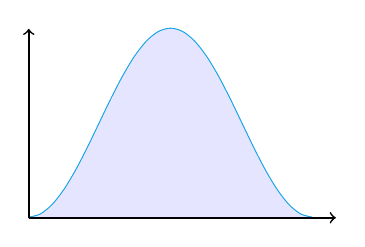
\begin{tikzpicture}[domain=0:6, scale=0.6]
        \draw[color=Cerulean, thick, smooth] plot (\x, {-2 * cos((\x / 6 * 2 * pi) r) + 2});
        \fill[color=blue!10, smooth] (0, 0) -- plot (\x, {-2 * cos((\x / 6 * 2 * pi) r) + 2}) -- (6, 0) -- cycle;

        \draw[semithick, ->] (0, 0) -- (6.5, 0);
        \draw[semithick, ->] (0, 0) -- (0, 4);
    \end{tikzpicture}
    \end{center}

    \item \textbf{Left Skewed Distribution}: One which has a peak on the right side and trails off down to the left.

    \begin{center}
    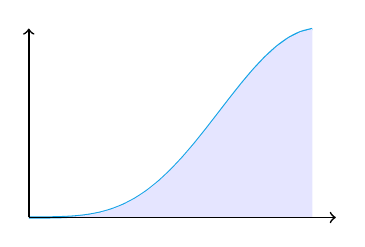
\begin{tikzpicture}[domain=0:6, scale=0.6]
        \draw[color=Cerulean, thick, smooth] plot (\x, {(sin((\x - 3) / 2 r) + 1)^2});
        \fill[color=blue!10] (0, 0) -- plot (\x, {(sin((\x - 3) / 2 r) + 1)^2}) -- (6, 0) -- cycle;

        \draw[semithick, ->] (0, 0) -- (6.5, 0);
        \draw[semithick, ->] (0, 0) -- (0, 4);
    \end{tikzpicture}
    \end{center}

    \item \textbf{Right Skewed Distribution}: One which has a peak on the left side and trails off down to the right.

    \begin{center}
    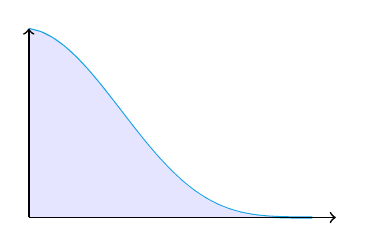
\begin{tikzpicture}[domain=0:6, scale=0.6]
        \draw[color=Cerulean, thick, smooth] plot (\x, {(-sin((\x - 3) / 2 r) + 1)^2});
        \fill[color=blue!10] (0, 0) -- plot (\x, {(-sin((\x - 3) / 2 r) + 1)^2}) -- (6, 0) -- cycle;

        \draw[semithick, ->] (0, 0) -- (6.5, 0);
        \draw[semithick, ->] (0, 0) -- (0, 4);
    \end{tikzpicture}
    \end{center}

    \item \textbf{Bimodal Distribution}: One which has peaks on both the right and left side, dropping down at the center.

    \begin{center}
    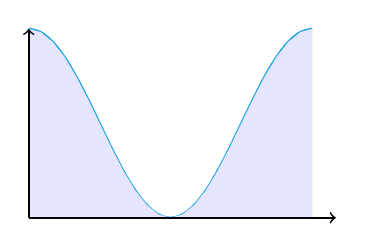
\begin{tikzpicture}[domain=0:6, scale=0.6]
        \draw[color=Cerulean, thick, smooth] plot (\x, {4 * cos((pi * \x / 6) r)^2});
        \fill[color=blue!10] (0, 0) -- plot (\x, {4 * cos((pi * \x / 6) r)^2}) -- (6, 0) -- cycle;

        \draw[semithick, ->] (0, 0) -- (6.5, 0);
        \draw[semithick, ->] (0, 0) -- (0, 4);
    \end{tikzpicture}
    \end{center}

    \item \textbf{Uniform Distribution}: One which is roughly consistent for all values.

    \begin{center}
    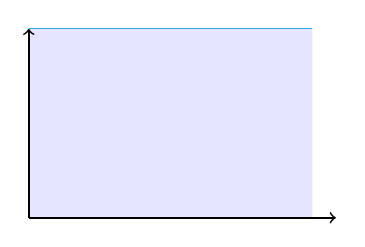
\begin{tikzpicture}[domain=0:6, scale=0.6]
        \draw[color=Cerulean, thick, smooth] plot (\x, {4});
        \fill[color=blue!10] (0, 0) -- plot (\x, {4}) -- (6, 0) -- cycle;

        \draw[semithick, ->] (0, 0) -- (6.5, 0);
        \draw[semithick, ->] (0, 0) -- (0, 4);
    \end{tikzpicture}
    \end{center}
\end{itemize}

There is also some more general terms that we can use to further describe parts of distributions.

\begin{blackbox}
    \begin{definition}
        A \textbf{cluster} is an area on the distribution where this a high
        amount or the majority of the data near this point. A \textbf{gap} is
        an area on the distribution where there is no data. This also goes in
        hand with \textbf{outliers}, which are data points offset from the
        general distribution, usually separated by gaps and found at the
        extremities. A \textbf{peak} as we have seen before is a high point on
        the distribution. The spread (or variability) of the graph can be
        described by the \textbf{range}, or the difference between the highest
        and lowest values in the data.
    \end{definition}
\end{blackbox}

Generally on the AP test and such when you're asked to \textit{describe} a
distribution, there are four major things you must find.

\begin{enumerate}
    \item \textbf{Shape}: These are described above (symmetric, left/right skewed, etc.).
    \item \textbf{Center}: This can be described with the mean or the median.
    \item \textbf{Spread}: These are described through the range, interquartile range, mean absolute deviation, standard deviation, etc. (These will come up later?)
    \item \textbf{Outliers}: Talk about whether there are or aren't any potential outliers in the data.
\end{enumerate}

When you're asked to \textit{compare} two or more distributions of data, look
at and compare the centers and spread.

Note that in some cases it is not always applicable to simply draw conclusions
based on the numerical values of the range and such, so be on the lookout and
intuit the information yourself.

\begin{blackbox}
    \begin{definition}
        The \textbf{IQR}, or \textbf{interquartile range}, of a given data set
        is found by taking the medians \( M_1 \) of upper half and \( M_2 \)
        lower half of the set and finding their difference \( M_1 - M_2 \).
        This is another measure of spread.
    \end{definition}
\end{blackbox}

\begin{example}
    The IQR of the data set \( 1, 1, 2, 5, 7, 8, 9 \) is \( 7 \). Because the
    median of \( 7, 8, 9 \) minus the median of \( 1, 1, 2 \) is \( 7 \).

    The IQR of the data set \( 2, 4, 6, 8 \) is \( 4 \) because the median of \( 6, 8 \) minus the median of \( 2, 4 \) is \( 4 \).
\end{example}

Often in statistics, we cannot take into account or measure data for an entire
population. In this case, we rely on taking \textbf{samples}, or smaller
groups, from this greater population and making generalizations to the entire
population based on the statistics from these smaller groups. When consider
samples however, we sometimes do have to make adjustments to how we interpret
summary statistics, in particular variance and standard deviation.

\begin{blackbox}
    \begin{definition}
        The \textbf{standard deviation} of an entire popluation with \( n \) data points, denoted by \( \sigma \), is given by the following:
        \[
            \sigma = \sqrt{\frac{\sum_{i = 1}^n \left( X_i - \mu  \right)^2}{n}},
        \]
        where \( X_i \) and \( \mu \) denote the \( i \)th value in population
        and the mean of the entire population, respectively.

        The \textbf{sample standard deviation}, however is slightly different. Let the mean of the sample be \( \overline{X} \) and the size be \( n \). Then the sample standard deviation, denoted with \( S \) is
        \[
            S = \sqrt{\frac{\sum_{i = 1}^n \left( X_i - \overline{X} \right)^2}{n - 1}}.
        \]

        To calculate variance, simply square the standard deviation.
    \end{definition}
\end{blackbox}

Notice the \( n - 1 \) in the denominator for the samples. This is used to
correct for bias in measurement.\footnote{Right now, the exact specifics as to
how and why are kind of fuzzy for me but here's a resource?
\url{https://stats.stackexchange.com/questions/3931/intuitive-explanation-for-dividing-by-n-1-when-calculating-standard-deviation}}

Generally when there exists outliers in the data, the median and interquartile
range are better choices for center and spread, while mean and standard
deviation are better for when there is more symmetric data without outliers.

Note we have that for any linear transformation \( T \colon X_i \mapsto a X_i +
b \) and set of data \( M \) the following (trivial to prove):
\begin{align*}
    \mu \left( T \left( M \right) \right) &= T \left( \mu \left( M \right) \right) \\
    \sigma \left( T \left( M \right) \right) &= a \left( \sigma \left( M \right) \right) \\
    \operatorname{Med} \left( T \left( M \right) \right) &= T \left( \operatorname{Med} \left( M \right) \right) \\
    \operatorname{IQR} \left( T \left( M \right) \right) &= a \operatorname{IQR} \left( M \right)
\end{align*}
In general, measures of centers should transform exactly under a linear
transformation, while measures of spread and range should only transform under
stretches (not translations).

\begin{blackbox}
    \begin{definition}
        When calculating these center and spread values for a \colorbox{Cerulean}{p}opulation we
        call them \textbf{\colorbox{Cerulean}{p}arameters}

        When we calculate them for a \colorbox{ForestGreen}{s}ample of the
        population, they are called \textbf{\colorbox{ForestGreen}{s}tatistics}.
    \end{definition}
\end{blackbox}

By convention, we consider any data point \( X \) an outlier when \( X < Q_1 -
1.5 \cdot IQR \) or \( X > Q_3 + \cdot 1.5 \cdot IQR \), where \( Q_1 \) and \(
Q_3 \) denote the first and third quartile respectively.

\begin{blackbox}
    \begin{definition}
        A \textbf{percentile} is defined as either the percentage of data below
        a certain value in the data, or the percentage of data below
        \textit{and including} a certain value in the data.
    \end{definition}
\end{blackbox}

\begin{example}
    The percentile rank of the value of \( 3 \) in the following data set is
    either \( 50\% \) or \( 75\% \) depending on definition\footnote{While the
        difference may seem large here, statisticians are fine with this
        somewhat lack of consensus on percentiles because the difference is
        quite negligible for large samples/populations}:
    \[
        1, 1, 3, 4
    .\]
\end{example}

This goes in tandem with cumulative relative frequency graphs.

\begin{blackbox}
    \begin{definition}
        A \textbf{cumulative relative frequency graph} is a graph that, given a
        corresponding \( x \)-value, tells one the percentage of values below
        that \( x \)-value in the set of data. This function, which we will denote \( f \left( x \right) \), is a strictly increasing bijection from the range of the data to the interval \( \left[ 0, 1 \right] \) such that \( f \left( a \right) = 0 \) and \( f \left( b \right) = 1 \).
    \end{definition}
\end{blackbox}

One very common tool in statistics is the notion of a \( z \)-score.

\begin{blackbox}
    \begin{definition}
        The \( z \)-score of a certain data point \( x \) is the number of
        standard deviations it is away from the mean. Numerically, that is:
        \[
            z = \frac{x - \mu}{\sigma}
        .\]
    \end{definition}
\end{blackbox}

This measure is used to tell us how often something occurs and can be useful to
help make inferences.

Oh boy it's time for some continuity now.

\begin{blackbox}
    \begin{definition}
        A \textbf{density function} or \textbf{density curve} is a continuous function \( f \left( x \right) \) defined on an interval \( \left[ a, b \right] \) such that
        \[
            \int_{a}^{b} f \left( x \right) \, dx = 1
        .\]
    \end{definition}
\end{blackbox}

\begin{center}
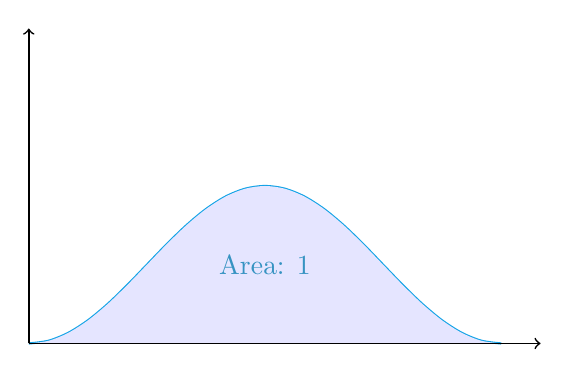
\begin{tikzpicture}[domain=0:6, scale=1]
    \draw[color=Cerulean, thick, smooth] plot (\x, {-1 * cos((\x / 6 * 2 * pi) r) + 1});
    \fill[color=blue!10, smooth] (0, 0) -- plot (\x, {-1 * cos((\x / 6 * 2 * pi) r) + 1}) -- (6, 0) -- cycle;

    \draw[semithick, ->] (0, 0) -- (6.5, 0);
    \draw[semithick, ->] (0, 0) -- (0, 4);

    \node[color=Cerulean!80!black] at (3, 1) {Area: \( 1 \)};
\end{tikzpicture}
\end{center}

This is the continuous equivalent of a relative frequency graph and allows us
to model data on a continuous spectrum of values and use our very nice tools of
analysis and such to describe what is going on. For instance, the area under
the curve in a specific interval (something given to us by the integral) gives
the density or probability of data being in the interval.

We can also determine median, mean, and skew graphically from these density
curves. The median line is one which splits the area of the curve exactly into
equal halves on each side, while the mean is the average value, or weighted
sum, of this curve. The location of where the mean and median line are relative
to each other determine the skew on the graph. When the mean is to the right of
the median, we call this right-skewed, and the other way around is called
left-skewed (terms we are already familiar with). For symmetric distributions,
the median and mean are roughly the same, meaning that they aren't skewed.

\begin{multicols}{3}
\begin{center}
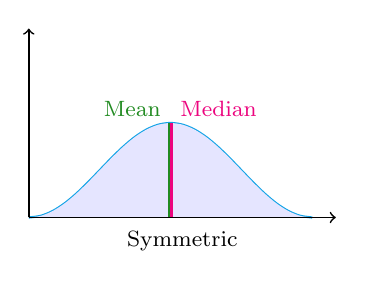
\begin{tikzpicture}[domain=0:6, scale=0.6]
    \draw[color=Cerulean, thick, smooth] plot (\x, {-1 * cos((\x / 6 * 2 * pi) r) + 1});
    \fill[color=blue!10, smooth] (0, 0) -- plot (\x, {-1 * cos((\x / 6 * 2 * pi) r) + 1}) -- (6, 0) -- cycle;

    \draw[very thick, color=ForestGreen] (2.975, 0) -- (2.975, 2);
    \draw[very thick, color=RubineRed] (3.025, 0) -- (3.025, 2);
    \node[anchor=east, color=ForestGreen] at (3, 2.3) {\footnotesize Mean};
    \node[anchor=west, color=RubineRed] at (3, 2.3) {\footnotesize Median};

    \draw[semithick, ->] (0, 0) -- (6.5, 0);
    \draw[semithick, ->] (0, 0) -- (0, 4);

    \node at (3.25, -0.5) {\footnotesize Symmetric};
\end{tikzpicture}
\end{center}

\begin{center}
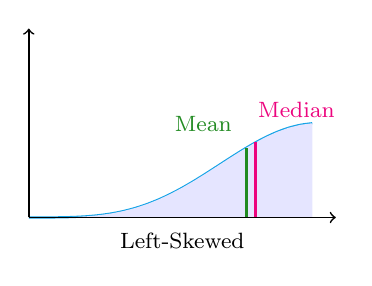
\begin{tikzpicture}[domain=0:6, scale=0.6]
    \draw[color=Cerulean, thick, smooth] plot (\x, {0.5 * (sin((\x - 3) / 2 r) + 1)^2});
    \fill[color=blue!10] (0, 0) -- plot (\x, {0.5 * (sin((\x - 3) / 2 r) + 1)^2}) -- (6, 0) -- cycle;

    \draw[very thick, color=ForestGreen] (4.60993567569, 0) -- (4.60993567569, 2.961 / 2);
    \draw[very thick, color=RubineRed] (4.797, 0) -- (4.797, 3.177 / 2);
    \node[anchor=east, color=ForestGreen] at (4.5, 2.961 / 2 + 0.5) {\footnotesize Mean};
    \node[anchor=west, color=RubineRed] at (4.65, 3.177 / 2 + 0.7) {\footnotesize Median};

    \draw[semithick, ->] (0, 0) -- (6.5, 0);
    \draw[semithick, ->] (0, 0) -- (0, 4);

    \node at (3.25, -0.5) {\footnotesize Left-Skewed};
\end{tikzpicture}
\end{center}

\begin{center}
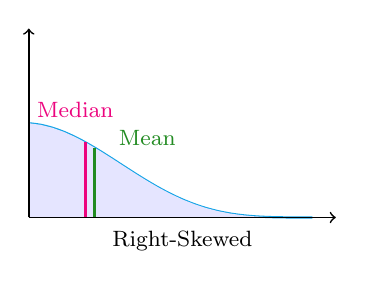
\begin{tikzpicture}[domain=0:6, scale=0.6]
    \draw[color=Cerulean, thick, smooth] plot (\x, {0.5 * (-sin((\x - 3) / 2 r) + 1)^2});
    \fill[color=blue!10] (0, 0) -- plot (\x, {0.5 * (-sin((\x - 3) / 2 r) + 1)^2}) -- (6, 0) -- cycle;

    \draw[very thick, color=ForestGreen] (6 - 4.60993567569, 0) -- (6 - 4.60993567569, 2.961 / 2);
    \draw[very thick, color=RubineRed] (6 - 4.797, 0) -- (6 - 4.797, 3.177 / 2);
    \node[anchor=west, color=ForestGreen] at (1.7, 2.961 / 2 + 0.2) {\footnotesize Mean};
    \node[anchor=east, color=RubineRed] at (2, 3.177 / 2 + 0.7) {\footnotesize Median};

    \draw[semithick, ->] (0, 0) -- (6.5, 0);
    \draw[semithick, ->] (0, 0) -- (0, 4);

    \node at (3.25, -0.5) {\footnotesize Right-Skewed};
\end{tikzpicture}
\end{center}
\end{multicols}

The normal distribution, or Gaussian distribution, is one of the most important
and prevalent distributions in statistics. The exact formulations will be
covered later, but the general sense is that it forms a symmetric bell curve shape.

One important idea surrounding the normal distribution is the empirical rule.

\begin{blackbox}
    \begin{definition}
        The \textbf{empirical rule}, or \textbf{\( \mathbf{68} \)-\( \mathbf{95} \)-\( \mathbf{99.7} \) rule} rule tells us that, for a normal distribution there is:
        \begin{itemize}
            \item A \( 68\% \) chance of a value being within one standard deviation of the mean,
            \item A \( 95\% \) chance of a value being within two standard deviations of the mean, and
            \item A \( 99.7\% \) chance of a value being within three standard deviations of the mean.
        \end{itemize}
    \end{definition}
\end{blackbox}

\vspace{0.3cm}

\begin{center}
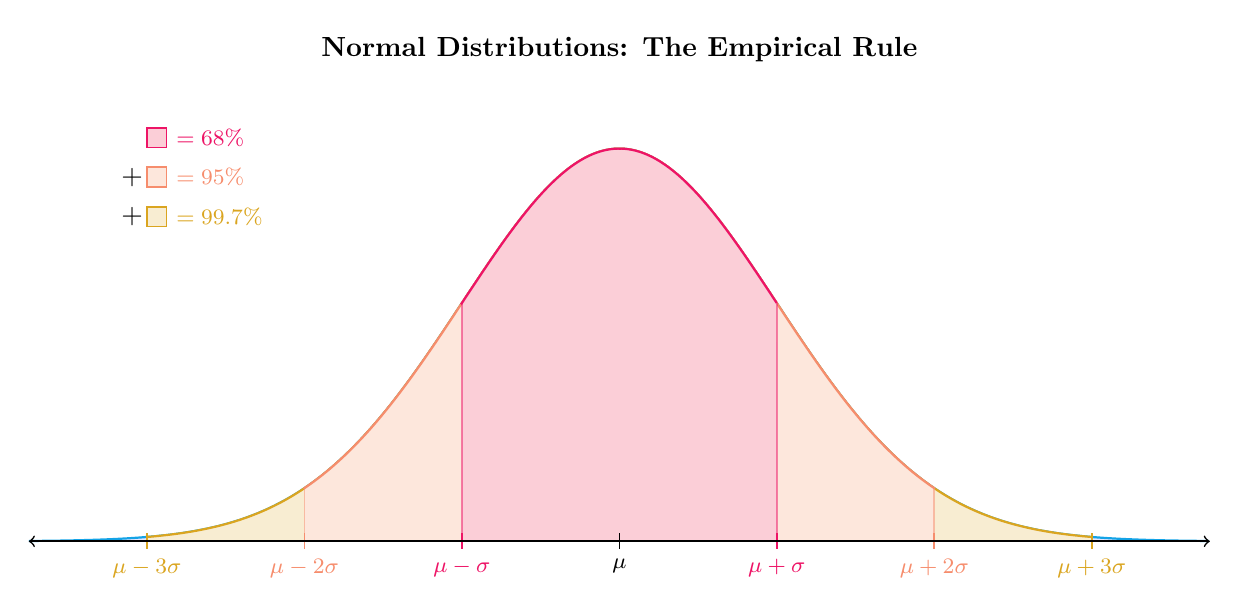
\begin{tikzpicture}[domain=-1.5:1.5, scale=5]
    \fill[color=blue!10, smooth] (-1.5, 0) -- plot (\x, {1/(0.4 * sqrt(2 * pi)) * exp(-1/2 * (\x / 0.4) ^ 2)}) -- (1.5, 0) -- cycle;
    \draw[color=Cerulean, thick, smooth, samples=200] plot (\x, {1/(0.4 * sqrt(2 * pi)) * exp(-1/2 * (\x / 0.4) ^ 2)});

    \fill[color=Goldenrod!20, smooth, domain=-1.2:1.2] (-1.2, 0) -- plot (\x, {1/(0.4 * sqrt(2 * pi)) * exp(-1/2 * (\x / 0.4) ^ 2)}) -- (1.2, 0) -- cycle;
    \draw[color=Goldenrod, thick, smooth, samples=200, domain=-1.202:1.202] plot (\x, {1/(0.4 * sqrt(2 * pi)) * exp(-1/2 * (\x / 0.4) ^ 2)});
    \draw[color=Goldenrod, semithick, draw opacity=0.5] (-1.2, 0) -- (-1.2, 0.0111);
    \draw[color=Goldenrod, semithick, draw opacity=0.5] (1.2, 0) -- (1.2, 0.0111);

    \fill[color=Melon!20, smooth, domain=-0.8:0.8] (-0.8, 0) -- plot (\x, {1/(0.4 * sqrt(2 * pi)) * exp(-1/2 * (\x / 0.4) ^ 2)}) -- (0.8, 0) -- cycle;
    \draw[color=Melon, thick, smooth, samples=200, domain=-0.802:0.802] plot (\x, {1/(0.4 * sqrt(2 * pi)) * exp(-1/2 * (\x / 0.4) ^ 2)});
    \draw[color=Melon, semithick, draw opacity=0.5] (-0.8, 0) -- (-0.8, 0.13498);
    \draw[color=Melon, semithick, draw opacity=0.5] (0.8, 0) -- (0.8, 0.13498);

    \fill[color=WildStrawberry!20, smooth, domain=-0.4:0.4] (-0.4, 0) -- plot (\x, {1/(0.4 * sqrt(2 * pi)) * exp(-1/2 * (\x / 0.4) ^ 2)}) -- (0.4, 0) -- cycle;
    \draw[color=WildStrawberry, thick, smooth, samples=200, domain=-0.402:0.402] plot (\x, {1/(0.4 * sqrt(2 * pi)) * exp(-1/2 * (\x / 0.4) ^ 2)});
    \draw[color=WildStrawberry, semithick, draw opacity=0.5] (-0.4, 0) -- (-0.4, 0.6049);
    \draw[color=WildStrawberry, semithick, draw opacity=0.5] (0.4, 0) -- (0.4, 0.6049);

    \draw[semithick] (0, 0.02) -- (0, -0.02) node[anchor=north] {\footnotesize \( \mu \)};

    \draw[semithick, color=WildStrawberry] (-0.4, 0.02) -- (-0.4, -0.02) node[anchor=north] {\footnotesize \( \mu - \sigma \)};
    \draw[semithick, color=WildStrawberry] (0.4, 0.02) -- (0.4, -0.02) node[anchor=north] {\footnotesize \( \mu + \sigma \)};

    \draw[semithick, color=Melon] (-0.8, 0.02) -- (-0.8, -0.02) node[anchor=north] {\footnotesize \( \mu - 2\sigma \)};
    \draw[semithick, color=Melon] (0.8, 0.02) -- (0.8, -0.02) node[anchor=north] {\footnotesize \( \mu + 2\sigma \)};

    \draw[semithick, color=Goldenrod] (-1.2, 0.02) -- (-1.2, -0.02) node[anchor=north] {\footnotesize \( \mu - 3\sigma \)};
    \draw[semithick, color=Goldenrod] (1.2, 0.02) -- (1.2, -0.02) node[anchor=north] {\footnotesize \( \mu + 3\sigma \)};

    \draw[semithick, <->] (-1.5, 0) -- (1.5, 0);

    \fill[color=WildStrawberry!20] (-1.2, 1.2 - 0.15) rectangle (-1.15, 1.15 - 0.15);
    \draw[semithick, color=WildStrawberry] (-1.2, 1.2 - 0.15) rectangle (-1.15, 1.15 - 0.15);
    \node[anchor=west, color=WildStrawberry] at (-1.2 + 0.05, 1.2 - 0.025 - 0.15) {\footnotesize \( = 68\% \)};

    \node at (-1.2375, 1.075 - 0.15) {\( + \)};
    \fill[color=Melon!20] (-1.2, 1.1 - 0.15) rectangle (-1.15, 1.05 - 0.15);
    \draw[semithick, color=Melon] (-1.2, 1.1 - 0.15) rectangle (-1.15, 1.05 - 0.15);
    \node[anchor=west, color=Melon] at (-1.2 + 0.05, 1.1 - 0.025 - 0.15) {\footnotesize \( = 95\% \)};

    \node at (-1.2375, 0.975 - 0.15) {\( + \)};
    \fill[color=Goldenrod!20] (-1.2, 1.0 - 0.15) rectangle (-1.15, 0.95 - 0.15);
    \draw[semithick, color=Goldenrod] (-1.2, 1.0 - 0.15) rectangle (-1.15, 0.95 - 0.15);
    \node[anchor=west, color=Goldenrod] at (-1.2 + 0.05, 1.0 - 0.025 - 0.15) {\footnotesize \( = 99.7\% \)};

    \node at (0, 1.25) {\textbf{Normal Distributions: The Empirical Rule}};
\end{tikzpicture}
\end{center}
% Hehe this took a while to make but hey it looks nice imo
